\documentclass{article}
\usepackage[utf8]{inputenc}
\usepackage[top=3cm, left=3cm, right=3cm, bottom=3cm]{geometry}
\usepackage[brazilian]{babel}
\usepackage{graphicx}

\makeatletter
\renewcommand\paragraph{\@startsection{paragraph}{4}{\z@}%
            {-2.5ex\@plus -1ex \@minus -.25ex}%
            {1.25ex \@plus .25ex}%
            {\normalfont\normalsize\bfseries}}
\makeatother
\setcounter{secnumdepth}{4} % how many sectioning levels to assign numbers to
\setcounter{tocdepth}{4}    % how many sectioning levels to show in ToC

\title{Aplicações de Álgebra Vetorial Linear em Computação}
\author{Eduardo Barreto Brito }
\date{November 2015}

\begin{document}

    \thispagestyle{empty}
    \begin{center}
        
\includegraphics[scale=0.01]{ufpe.png}\\
        \large{{\sc Universidade Federal de Pernambuco}}
    \end{center}
    \vspace{7cm}
    \hrulefill
    \begin{center}
        \large{ \ {\bf ÁLGEBRA VETORIAL LINEAR PARA COMPUTAÇÃO}}\\[0.2cm]
        \large{\textsf{Aplicações de Álgebra Vetorial Linear em PDI}}\\
    \end{center}
    \hrulefill\\[3.4cm]
    \begin{center}
        \textsc{Alan Bezerra da Silva}\\
        \textsc{Eduardo Barreto Brito}\\
        \textsc{Lucas Augusto de Mota Alcântara}\\
        \textsc{Lucas Pontes de Albuquerque}\\
        \textsc{Miguel Luiz Pessoa da Cruz Silva}\\
        \textsc{Vladson Henrique Ribeiro Marinho}
    \end{center}
    \vspace{2.6cm}
    \textsc{Recife, Novembro de 2015}\\
    {\bf Professor:} Paulo Salgado
    \newpage
    \tableofcontents
    \newpage

    \section{O que é Álgebra Vetorial Linear?}
        Álgebra Vetorial Linear (AVL) é o ramo da matemática que estuda espaços vetoriais, espaços lineares e funções lineares, que relacionam vetores entre dois ou mais espaços. Em outras palavras, a Álgebra Vetorial Linear tenta representar o cotidiano através de formas algébricas e achar relações lineares entre elas.
    
    \section {Qual sua aplicação na Computação?}
        Por se tratar da representação do cotidiano algebricamente, é na computação que Álgebra Vetorial Linear mais demonstra influência, ou seja, em mais campos ela se apresenta.\\        
        Na computação gráfica, por exemplo, a manipulação de imagens, rotação, redimensionamento, alteração de cores são operações lineares. Até mesmo as imagens que vemos em nossos monitores ou projetores, que são medidos por Pixels, são representados, na computação, por matrizes.\\     
        Ainda dentro de computação gráfica, a parte de PDI (Processamento Digital de Imagem) é, basicamente Álgebra Vetorial. Utilizando de Matrizes e mudanças de bases, é possível melhorar (ou piorar) a situação de uma imagem, além de alterá-la automaticamente, simplesmente mudando a matriz que dá origem a base de cores utilizadas pela imagem.\\        
        Além disso, outros exemplos de processos que usam álgebra são: criação de objetos em 3 dimensões através de matrizes, aplicação de textura plana ao objeto em 3 dimensões, cálculo para descobrir o ponto certo para a aplicação de sombras aos objetos em 3D, cálculo de rota (Sistemas de roteirização) e aproximação de comportamentos não lineares com sistemas lineares, otimizando-os, através de programas que os transformam em gráficos.
    
    \section {Aplicações de Álgebra Linear Vetorial em PDI}
        
        \subsection {O que é PDI?}
        Processamento Digital de Imagens (PDI) pode ser compreendido como uma ``manipulação de uma imagem por um computador de modo que a entrada e a saída do processo sejam imagens'' (4). Ou seja, é um processo virtual no qual é inserida uma imagem e o computador executa uma serie de processos naquela figura a fim de transformá-la de algum modo, ``devolvendo'' uma imagem processada.\\
        O objetivo do Processamento Digital de Imagens é facilitar ao máximo a interpretação de imagens. As formas que usamos para manipular as imagens são, essencialmente, infinitas, porém podem ser classificadas em procedimentos que incluem quatro tipos abrangentes de operações computacionais\footnote{As classificações foram tiradas de (4)}:
        
        \begin {enumerate}
            
            \item Retificação e Restauração de Imagens: operações realizadas para minimizar as distorções e degradações dos dados de uma imagem, com a finalidade de criar uma representação mais fiel da cena;
            
            \item Realçamento de Imagens: procedimentos aplicados aos dados de uma imagem com o objetivo de melhorar efetivamente a visualização da cena, para subseqüente interpretação visual;
            
            \item Classificação de Imagens: estas operações têm a finalidade de substituir a análise visual dos dados por técnicas quantitativas de análise automática, visando a identificação das regiões presentes na cena;
            
            \item Combinação de Dados ({\it data merging}): procedimentos utilizados para combinar os dados de uma imagem, referente a uma certa área geográfica, com outros conjuntos de dados referenciados geograficamente, para a mesma área.
       
        \end {enumerate}
        
        
        \subsection {Aplicações de AVL em PDI}
        Uma imagem é formada por uma \textit{matriz}, onde cada posição dessa matriz possui informações dela, como, por exemplo, a cor, iluminação (quantidade de luz incidindo na cena, que é determinada pela fonte de luz)  e reflectância (quantidade de luz refletida pelos objetos na cena, que é determinada pelas características dos objetos na cena). Cada posição da matriz que carrega informações desse tipo é chamada de \textit{pixel}. A quantidade de pixels de uma imagem define sua \textit{resolução}.\\
        Cada pixel tem 8 posições vizinhas a ele, que são utilizadas para análise nos processos que modificam a imagem. O conjunto de todos esses ``8 vizinhos'' é chamado de {\it 8-vizinhança}. Ou seja, as informações de uma imagem, que são {\it processadas}, são interpretadas todas através de uma {\it matriz}, independente de quão grande ela seja.
        
            \subsubsection {Operações com as matrizes}
                
                \paragraph {Adição para redução de ruído}
                    Se tivermos várias fotos diferentes de uma mesma cena, todas com qualidade insatisfatória, apresentando ruídos aleatórios, ao somarmos as matrizes que correspondem àquelas imagens, teremos no final uma imagem com uma qualidade melhor, apesar de apresentar, no fim, cores mais fortes que a imagem original. Isso acontece porque os ruídos são falhas na captura de imagem e, por serem aleatórios, ao somarmos, as posições que correspondem à cor original da imagem começará a surgir no lugar do que seriam os ruídos das outras imagens, diminuindo a {\it quantidade de ruído} da mesma.

                \paragraph{Subtração na detecção de movimento}
                    Ao subtrairmos as matrizes de várias fotos de uma mesma cena onde aconteceu um movimento, as posições que não apresentaram modificações são posições que indicam pixels que não mudaram, ou seja, posiçãos que não se movimentaram, irão zerar. Por outro lado, as posições que foram modificadas pouco alterarão seus valores, o que gerarão um rastro por onde o objeto se movimentou, {\it explicitando o trajeto} do mesmo.
                    
                \paragraph{Operações locais ou de vizinhança {\it (neighbourhood)}}
                    Operações locais ou de vizinhança são funções aplicadas nos pixels que também se aplica aos pixels vizinhos.
                    
                \paragraph {Operações geométricas}
                    Nas operações geométricas, separa-se os pixels, aumentando a ``distância'' entre eles e, ao separar, replica os pixels originais em seus vizinhos, preenchendo as posiçoes vazias geradas pela separação dos pixels originais. Resulta em um {\it zoom} da imagem.
                    
            \subsubsection{O Filtro Mediana}
                Esse filtro {\it ordena os pixels de forma crescente e retorna o pixel central da matriz quadrada de tamanho arbitrado}. Ajuda muito a reduzir os ruídos localizados por grande diferença de intensidade.
                
            \subsubsection{Domínios}
                
                \begin{enumerate}
                
                \item Domínio espacial: se refere ao plano da imagem que contém as {\it intensidades} dos pixels;
                
                \item Domínio da frequência: é ``a análise de funções matemáticas com respeito à {\it frequência}, em contraste com a análise no domínio do tempo.'' (5)
                
                \end{enumerate}
                
                \paragraph{Domínio Espacial}
                    No Domínio Espacial, isto é, se tratando a matriz que representa a imagem propriamente dita, pode se realizar várias operações a fim de atingir um resultado mais sastisfatório que o original. A esse conjunto de operações se dá o nome de Realce no Domínio Espacial. São exemplos: Filtragem Espacial, Máscaras com vizinhança 1x1 e processamento ponto-a-ponto, mapeamento, funções: linear, logarítimica, potência e negativa de intensidade. Outros exemplos de Realce no Domínio Espacial são Alargamento de contraste, fatiamento de níveis de intensidade e Fatiamento de planos de bits. Como todas essas operações são no Domínio Espacial, todas se utilizam dos conceitos de AVL relacionados à matrizes.\\
                    O {\it histograma} (O histograma de uma imagem digital com níves de cinza é uma função discreta h(rk) = nk, onde rk é o k-ésimo nível de cinza, e nk é o número total de pixel na imagem com esse nível de cinza) é uma forma de representar uma imagem no Domínio Espacial e sua manipulação é útil para realce e para fornecer estatísticas da imagem. Como o histograma é uma representação dos pixels da imagem e, por sua vez, os pixels são as posições da matriz que corresponde a imagem, uma alteração no histograma alteraria, por consequência, a matriz que define a imagem, modificando-a. O histograma pode ser realçado através de Equalização, Especificação, Localmente, e pode ser usado como Estatística.
                \paragraph{Filtros Espaciais}
                Os Filtros Espaciais são filtros (série de operações) aplicadas ao Domínio Espacial. São eles:
                
                \begin{enumerate}
                
                \item Filtros Espaciais de Suavização ({\it Smoothing Spatial Filters}): usados para borramento e redução de ruído;
                
                \item Filtros Espaciais de Aguçamento ({\it Sharpening Spatial Filters}): usados para enfatizar uma parte da imagem, ou seja, dar destaque a uma pedaço específico;
                
                \end{enumerate}
                Esses filtros podem ser combinados com o intuito de gerar uma imagem ainda mais satisfatória para um uso específico.
                
                \paragraph{Domínio da Frequência}
                    Assim como no Domínio Espacial, também é possível aplicar operações de Realce no Domínio da Frequência. As operações no Domínio da Frequência vêm de operações com {\it Séries e Transformadas de Fourier\footnote{Definição em Informações Extras}} do Domínio Espacial. Grande parte dessas operações dependem de conceitos relacionados à matrizes, já que se utiliza a representação 2D da Transformada Discreta de Fourier e a centralização da mesma.\\
                    
                \paragraph{Filtros no Domínio da Frequência}
                    Em relação à filtragem no Domínio da Frequência, existem três tipos:
                    
                    \begin{enumerate}
                    
                    \item Filtros passa-baixa, que preserva as baixas frequências espaciais\footnote{Area de suavização} e suprime as altas frequências espaciais\footnote{Detalhes, como bordas e ruídos} , suavizando e/ou borrando da imagem;
                    
                    \item Filtros passa-alta, que preserva as altas frequências espaciais e suprime as baixas frequências espaciais, realçando as bordas e/ou aguçando a imagem;
                    
                    \item Filtros passa-faixa, preserva específicas frequências espaciais e suprime outras frequências espaciais, restaurando a imagem.
                
                    \end{enumerate}
                Um exemplo de filtro do Domínio da Frequência é o Filtro Ideal, que define um círculo no qual todas as frequências dentro dele passam sem alterações, o que permite que ele seja utilizado tanto como passa-baixa quanto como passa-alta. O mesmo serve para os filtros de Butterworth e Gaussiano. 
                     
            \subsubsection{Processamento de Imagem Morfológica}
            A Linguagem da Morfologia, aos olhos da matemática, é a Teoria dos Conjuntos. E o conjunto de todos os pixels pretos em uma imagem binária é uma descrição completa dessa imagem.
                \paragraph{Operadores morfológicos fundamentais}
                
                \begin{enumerate}
                
                \item Dilatação de A por B\footnote{Tirado de (7)}: transformação linear que obtém a reflexão de B em torno de sua origem, seguido da translação dessa reflexão por x; 
                
                \item Erosão\footnote{Tirado de (7)}: A erosão de A por B é o conjunto de todos os pontos x tais que B, quando transladado pro x fique contido em A.
                
                \end{enumerate}
                
            \subsubsection{Segmentação}
            A segmentação divide a imagem em suas partes ou objetos que a constituem. O que define como dividir a imagem são os níveis de cinza, que tem seu comportamento dividido em:
            
            \begin{enumerate}
            
            \item Descontinuidade: diferença súbita e grande nos níveis de cinza. Consegue detectar pontos isolados, linhas e bordas;
            
            \item Similaridade: analisa continuidade de crescimento/decrescimento dos niveis de cinza, detectando regiões que eles são semelhantes ou possuem valores próximos. Divide e funde regiões.
            
            \end{enumerate}
            Ambos os modos de segmentar a imagem são baseados na ideia de ``8-vizinhança'' das posições da matriz, ou seja, dos pixels.\\
            Após a segmentação da imagem, vem a parte de Reconhecimento. A partir das informações encontradas pela segmentação, os objetos são reconhecidos e definidos.
            
            \subsubsection{Processamento de Imagens Coloridas}
            Nessa seção de PDI, além da utilização de operações com as matrizes, o conceito de Mudança de Bases também é utilizado. Aplicando-o, podemos trocar a base das cores da imagem que está sendo processada, realçando ou desperdiçando dados que são importantes ou inúteis, respectivamente. Os principais modelos de cores são:
            
            \begin{enumerate}
            
            \item RGB: {\it Red, Green, Blue} (vermelho, verde e azul, respectivamente);
            
            \item CMY: {\it Cyan, Magenta, Yellow} (ciano, magenta e amarelo, respectivamente);
            
            \item CMYK: CMY com o preto adicionado;
            
            \item HSI: {\it Hue, Saturation, Intensity} (matiz, saturação e intensidade). A matiz representa o conceito de cor em relação ao vermelho, saturação indica a proporção de luz branca na cor e intensidade representa a distância da cor ao preto.
            
            \end{enumerate}
            Para aumentar as aplicações de PDI e aumentar a possibilidade de efeitos especiais, é usado uma técnica que analisa uma imagem por meio de várias imagens, dependendo da base de cores utilizadas. Por exemplo, se estiver usando a base de cores RGB, separa-se a imagem em tons de {\it Red} (vermelho), tons de {\it Green}(verde) e tons de {\it Blue} (azul), modifica cada uma e depois junta todas novamente.\\
            Ao mudar a base dos modelos das cores através do conceito de Mudança de Bases, a imagem tem suas cores alteradas drásticamente. Exemplos de mudanças são:
            
            \begin{enumerate}
            
            \item De CMY para RGB: 
            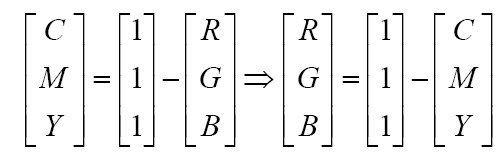
\includegraphics[scale=0.4]{CMYparaRGB.jpg}
            
            \item De RGB para CMYK:
            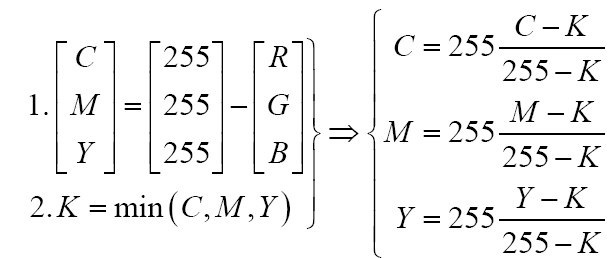
\includegraphics[scale=0.4]{RGBparaCMYK.jpg}
            
            \end{enumerate}
        
        \subsection{Curiosidade: detectando um QR Code}
            \subsubsection{O que é um QR Code?}
            {\it Quick Response Code}: Uma espécie de código de barras em matriz, que tornou-se bastante popular pela sua velocidade de leitura e grande capacidade de armazenamento.
            
            \subsubsection{Como detectar a existência do QR Code?}
            A detecção de um QR Code consiste na ideia de identificar {\it Finder Patterns\footnote{Pequenos quadrados em preto e branco localizados na extremidade do QR Code}}.
            
            \subsubsection{Encontrando um QR code}
                \paragraph{Pré-processamento}
                Antes de iniciar o processamento da imagem para identificar a existência de um QR Code, fazemos dois passos considerados inicias:
                
                \begin{enumerate}
                
                \item Converter imagem para tons de cinza;
                
                \item Binarizar imagem.
                
                \end{enumerate}
                
                \paragraph{Achando os Finder Patterns}
                É possível observar que existe uma proporção no número de preto/branco/preto/branco/preto que se mantém a mesma, não importa o ângulo (1:1:3:1:1, respectivamente). Após perceber isso, é só seguir os passos:
                
                \begin{enumerate}
                
                \item Ler toda a imagem buscando a proporção padrão;
                
                \item Salvar os possíveis centros de um Finder Pattern;
                
                \item Caso encontre mais do que 3 pontos, selecionar apenas 3 para serem os pontos do Finder Pattern;
                
                \item De posse da imagem binarizada, utilizar findContours()\footnote{Comando do Matlab} que retorna todos os contornos da imagem;
                
                \item Eliminar contornos irrelevantes;
                
                \item Encontrar contornos que estão dentro dos outros;
                
                \item Eliminar contornos fora da proporção para um Finder Pattern;
                
                \item Os que sobrarem, são Finder Patterns;
                
                \item Por fim, extração do QR Code: Transformação Linear (getAffineTransform()\footnote{Comando do Matlab} e warpAffine()\footnote{Comando do Matlab}).
                
                \end{enumerate}
                
            \subsection{Intenção da curiosidade}
            QR Code é algo utilizado por muitos no dia a dia ({\it Whatsapp Web}, por exemplo) e, para lê-los, é necessário utilizar de vários processos e comandos que utilizam conceitos estudados por AVL, comprovando mais uma vez o quão grande é o leque de aplicações de AVL na computação. Toda a seção de curiosidade foi retirada de (10).
            
            \subsection{Aplicação {\it indireta} de AVL em PDI}
        O {\it Matlab} é um dos programas mais utilizados em PDI. Este programa consegue realizar as operações e grande parte das funções necessárias para a alteração de imagens.\\
        Apesar de ser completo, o Matlab utiliza de conceitos relativamente simples, que estão presentes em AVL. Conceitos como Vetores, Matrizes, Transformações Lineares através de funções são muito utilizados nele, exemplificando, mais uma vez, a grande abrangência de AVL em Computação.
         
        \subsection{Informações Extras}
        Série de Fourier é uma forma de representação de uma função periódica como uma soma de funções de senos e cossenos e transformada de Fourier é aplicada para funções não periódicas.

                
        
    \newpage
    
    \section{Bibliografia}
        
        \begin{enumerate}
        
        \item ``Aplicações de Álgebra Vetorial Linear na Computação'', ROBERTO MARQUES DE JESUS,\\Paulo. 13 de Julho de 2013. Disponível em: \textless http://pauloinfotech.blogspot.com.br/2013/07/a\\plicacoes-algebra-linear-computacao.html\textgreater. Acesso: 01 de Novembro de 2015.
        
        \item ``Aplicações Práticas'', autor desconhecido. Disponível em: \textless http://www.mat.ufmg.br/gaal/apl\\icacoes/aplicacoes.html\textgreater. Acesso: 01 de Novembro de 2015.
        
        \item ``Programação Linear'', Wikipedia. 31 de Outubro de 2015. Disponível em:
        \textless https://pt.wikipedia\\.org/wiki/Programa\%C3\%A7\%C3\%A3o\_linear\textgreater. Acesso: 01 de Novembro de 2015.
        
        \item ``Processamento Digital de Imagens'', autor desconhecido. Disponível em: \textless http://www.ufrgs.br/\\engcart/PDASR/pdi.html\textgreater. Acesso: 14 de Novembro de 2015.
        
        \item ``Domínio da Frequência'', Wikipedia. 14 de Dezembro de 2014. Disponível em: \textless https://pt.wikip\\edia.org/wiki/Dom\%C3\%ADnio\_da\_frequ\%C3\%AAncia \textgreater. Acesso: 15 de Novembro de 2015.
        
        \item Doc. Powerpoint de aulas de Processamento Digital de Imagens, por Bruno Fernandes. ECOMP-POLI 2015.1.
        
        \item Doc. Powerpoint da aula de Processamento de Imagem Morfológica (Morfologia Matemática), por Tsang Ing Ren. CIn-UFPE.
        
        \item Doc. Powerpoint da aula de Segmentação, por Tsang Ing Ren. CIn-UFPE.
        
        \item Doc. Powerpoint da aula de Processamento de Imagens Coloridas, por Tsang Ing Ren. CIn-UFPE.
        
        \item ``Projeto QR Code'', BARRETO BRITO, Hartur e RIBEIRO, Thiago. Junho de 2015. ECOMP-POLI 2015.1. Acesso: 15 de Novembro de 2015.
        
        \item ``INTRODUÇÃO AO PROCESSAMENTO DIGITAL DE IMAGENS'', MAILARD, Philippe. 2001. Disponível em: \textless http://csr.ufmg.br/geoprocessamento/publicacoes/cursopdi.pdf\textgreater. Acesso: 15 de Novembro de 2015.
        
        \end{enumerate}

\end{document}
